% !TEX TS-program = XeLaTeX
% use the following command:
% all document files must be coded in UTF-8
\documentclass[english]{textolivre}
% build HTML with: make4ht -e build.lua -c textolivre.cfg -x -u article "fn-in,svg,pic-align"

\journalname{Texto Livre}
\thevolume{17}
%\thenumber{1} % old template
\theyear{2024}
\receiveddate{\DTMdisplaydate{2023}{7}{10}{-1}} % YYYY MM DD
\accepteddate{\DTMdisplaydate{2023}{8}{1}{-1}}
\publisheddate{\DTMdisplaydate{2023}{12}{4}{-1}}
\corrauthor{Edison Ferney Castrillón Ángel}
\articledoi{10.1590/1983-3652.2024.46827}
%\articleid{NNNN} % if the article ID is not the last 5 numbers of its DOI, provide it using \articleid{} commmand 
% list of available sesscions in the journal: articles, dossier, reports, essays, reviews, interviews, editorial
\articlesessionname{articles}
\runningauthor{Castrillón Ángel and Rodrigues} 
%\editorname{Leonardo Araújo} % old template
\sectioneditorname{Daniervelin Pereira}
\layouteditorname{João Mesquista}

\title{Media as a critical pedagogy scenario to promote reexistence literacies with pre-service English teachers}
\othertitle{Mídia como um cenário de pedagogia crítica para promover letramentos de reexistência com professores de inglês em formação}
% if there is a third language title, add here:
%\othertitle{Artikelvorlage zur Einreichung beim Texto Livre Journal}

\author[1,2]{Edison Ferney Castrillón Ángel~\orcid{0000-0001-9237-1084}\thanks{Email: \href{mailto:edison.castrillonan@gmail.com}{edison.castrillonan@gmail.com}}}
\author[1]{Beatriz Gama Rodrigues~\orcid{0000-0001-8802-8320}\thanks{Email: \href{mailto:beatriz@ufpi.edu.br}{beatriz@ufpi.edu.br}}}
\affil[1]{Universidade Federal do Piauí, Letras, Teresina, PI, Brasil.}
\affil[2]{Universidad Católica Luís Amigó, Medellín, Colômbia.}

\addbibresource{article.bib}
% use biber instead of bibtex
% $ biber article

% used to create dummy text for the template file
\definecolor{dark-gray}{gray}{0.35} % color used to display dummy texts
\usepackage{lipsum}
\SetLipsumParListSurrounders{\colorlet{oldcolor}{.}\color{dark-gray}}{\color{oldcolor}}

% used here only to provide the XeLaTeX and BibTeX logos
\usepackage{hologo}

% if you use multirows in a table, include the multirow package
\usepackage{multirow}

% provides sidewaysfigure environment
\usepackage{rotating}

%UsepackageS to improve and create better tables
\usepackage{tabularx}


% CUSTOM EPIGRAPH - BEGIN 
%%% https://tex.stackexchange.com/questions/193178/specific-epigraph-style
\usepackage{epigraph}
\renewcommand\textflush{flushright}
\makeatletter
\newlength\epitextskip
\pretocmd{\@epitext}{\em}{}{}
\apptocmd{\@epitext}{\em}{}{}
\patchcmd{\epigraph}{\@epitext{#1}\\}{\@epitext{#1}\\[\epitextskip]}{}{}
\makeatother
\setlength\epigraphrule{0pt}
\setlength\epitextskip{0.5ex}
\setlength\epigraphwidth{.7\textwidth}
% CUSTOM EPIGRAPH - END

% LANGUAGE - BEGIN
% ARABIC
% for languages that use special fonts, you must provide the typeface that will be used
% \setotherlanguage{arabic}
% \newfontfamily\arabicfont[Script=Arabic]{Amiri}
% \newfontfamily\arabicfontsf[Script=Arabic]{Amiri}
% \newfontfamily\arabicfonttt[Script=Arabic]{Amiri}
%
% in the article, to add arabic text use: \textlang{arabic}{ ... }
%
% RUSSIAN
% for russian text we also need to define fonts with support for Cyrillic script
% \usepackage{fontspec}
% \setotherlanguage{russian}
% \newfontfamily\cyrillicfont{Times New Roman}
% \newfontfamily\cyrillicfontsf{Times New Roman}[Script=Cyrillic]
% \newfontfamily\cyrillicfonttt{Times New Roman}[Script=Cyrillic]
%
% in the text use \begin{russian} ... \end{russian}
% LANGUAGE - END

% EMOJIS - BEGIN
% to use emoticons in your manuscript
% https://stackoverflow.com/questions/190145/how-to-insert-emoticons-in-latex/57076064
% using font Symbola, which has full support
% the font may be downloaded at:
% https://dn-works.com/ufas/
% add to preamble:
% \newfontfamily\Symbola{Symbola}
% in the text use:
% {\Symbola }
% EMOJIS - END

% LABEL REFERENCE TO DESCRIPTIVE LIST - BEGIN
% reference itens in a descriptive list using their labels instead of numbers
% insert the code below in the preambule:
%\makeatletter
%\let\orgdescriptionlabel\descriptionlabel
%\renewcommand*{\descriptionlabel}[1]{%
%  \let\orglabel\label
%  \let\label\@gobble
%  \phantomsection
%  \edef\@currentlabel{#1\unskip}%
%  \let\label\orglabel
%  \orgdescriptionlabel{#1}%
%}
%\makeatother
%
% in your document, use as illustraded here:
%\begin{description}
%  \item[first\label{itm1}] this is only an example;
%  % ...  add more items
%\end{description}
% LABEL REFERENCE TO DESCRIPTIVE LIST - END


% add line numbers for submission
%\usepackage{lineno}
%\linenumbers

\begin{document}
\maketitle

\begin{polyabstract}
\begin{abstract}
This study aims to reveal how media, as a critical pedagogy scenario \cite{apple1990,mclaren2007critical}, can promote reexistence literacies, through the development of resistance narratives \cite{kleiman2016,silva-souza2009letramentos}. It is a Qualitative Online Research (QOR) \cite{denzin2005} focused on the sociocritical paradigm \cite{freire1970} and Young Participatory Action Research \cite{mirra2015doing}. We conducted this study through an online media course composed of 18 sessions, with 18 preservice English teachers from Universidade Federal do Piauí (located in the northeast of Brazil) and Universidad Católica Luis Amigó (located in Medellín, Colombia). The research evidences that: a) the majority of the pre-service English teachers reveal some lack of awareness concerning the critical use and consumption of information in communication means; b) the development of reexistence literacies occurs when the individuals are conscious and empower themselves in their scenarios to fight for a world with more justice and equity; c) Reexistence may occur when critical pedagogical practices of resistance are employed. In conclusion, we highlight the importance of using the media to question power structures, promote critical education for equity, and generate scenarios for the active participation of teachers and students to promote the development of reexistence literacies through resistance narratives.

\keywords{Resistance narratives \sep Reexistence literacies \sep Digital media \sep Critical pedagogy \sep Linguistic and cultural education}
\end{abstract}

\begin{portuguese}
\begin{abstract}
Este estudo tem como objetivo revelar como a mídia, como um cenário de pedagogia crítica \cite{apple1990,mclaren2007critical}, pode promover letramentos de reexistência, por meio do desenvolvimento de narrativas de resistência \cite{kleiman2016,silva-souza2009letramentos}. Trata-se de uma Pesquisa Qualitativa Online (PQO) \cite{denzin2005} voltada para o paradigma sociocrítico \cite{freire1970} e Pesquisa-Ação Participativa Jovem \cite{mirra2015doing}. Conduzimos este estudo por meio de um curso de mídia on-line composto por 18 sessões, com 18 professores de inglês em formação da Universidade Federal do Piauí (localizada no nordeste do Brasil) e da Universidad Católica Luis Amigó (localizada em Medellín, Colômbia). A pesquisa evidencia que: a) a maioria dos professores de inglês em formação revela alguma falta de consciência quanto ao uso e consumo crítico da informação nos meios de comunicação; b) o desenvolvimento de letramentos de reexistência ocorre quando os indivíduos se conscientizam e se empoderam em seus cenários para lutar por um mundo com mais justiça e equidade; c) a reexistência pode ocorrer quando práticas pedagógicas críticas de resistência são empregadas. Em conclusão, destacamos a importância de usar a mídia para questionar as estruturas de poder, promover a educação crítica para a equidade e gerar cenários para a participação ativa de professores e alunos para promover o desenvolvimento de letramentos de reexistência por meio de narrativas de resistência.

\keywords{Narrativas de resistência \sep Letramentos de reexistência \sep Mídia digital \sep Pedagogia crítica \sep Educação linguística e cultural}
\end{abstract}
\end{portuguese}
\end{polyabstract}

\section{Introduction}\label{sec-intro}

In a society in which so many people are minoritised every day in social, academic, and political contexts, we should, as educators attempt to include more criticality in linguistic education. When we consider teaching education, more specifically pre-service language teachers, this consciousness may have a more relevant significance. As English language professors, we constantly discuss and redefine the importance of critical pedagogies and decoloniality in teaching and research.

Considering these issues, this qualitative online study presents an alternative approach to understanding media as platforms to promote reexistence literacies among pre-service English teachers. This research emerged after recognising the importance of empowering students to challenge stereotypes, prejudices, and acts of oppression and injustice that they or their communities face. Through this endeavor, the learning and teaching of the English language go beyond mere mechanical linguistic scopes, becoming an opportunity for each pre-service teacher to read and comprehend their world through physical and digital contexts, thereby proposing socio-cultural actions that lead to a more just and equitable environment.

The study highlights reexistence literacy as a capacity and ability that humans develop to liberate themselves from the influences of colonisation in their existence, perceptions, communication, and imagination, asserting their right to occupy a position of respect and honor in society \cite{alban2017,silva-souza2009letramentos,opendemocracy2022resistencia}. Similarly, it demonstrates how media can become platforms for either liberation or oppression, depending on individuals’ ability to develop critical skills that enable them to validate the accuracy, reliability, and quality of the information they receive or disseminate.

This study involved two different populations from the English Letters and Foreign Language Education programs at the Universidade Federal do Piauí in Teresina, Brazil, and the Universidad Católica Luis Amigó in Medellín, Colombia. Using the principles of young participatory action research, we designed and implemented a media project consisting of 18 online sessions divided into four stages. We also employed various techniques during these stages to generate qualitative data that might help us understand and identify participants’ perceptions of their family, work, and academic contexts, as well as their difficulties in creating and sharing narratives within the media project.

In this text, we present the scope and limitations of this research, highlighting that projects utilising digital media offer an interactive space for individuals to actively participate in thoughtful discussions, delve into intricate subjects, and question prevailing systems of authority. Moreover, it underscores the potential of education as a vehicle for promoting fairness, resilience, and reexistence, creating possibilities for inclusivity and metamorphosis, nurturing cultural identity, empowering communities, and cultivating socio-political consciousness.

\section{Theoretical support}\label{sec-theoret}
\subsection{Resistance}\label{subsec-resist}
Resistance becomes a fighting action, a skill that many people in Latin America and many other parts of the world have developed because of the injustices and abuses that have been established in their contexts. Thanks to this action, today there are still different cultures such as the palenquera in Colombia that, thanks to their resistance, became the first free town in America that fled slavery in colonial times \cite{larepublica2022}. Through resistance, the Munduruku, in Brazil, have been able to survive the abuses of state power and protect their 130 villages from colonialism \cite{opendemocracy2022resistencia}. Thanks to resistance, thousands of women today can have the popular vote in many countries where only a few years ago only men voted. Due to resistance, many men and women today can be and exist in their worlds. For that reason, resistance is necessary to survive and not die.

For authors such as \textcite{giroux1983}, resistance requires broader theoretical issues such as power and agency. Power is held by dominant groups and is used to oppress and eliminate cultures and identities. From there, the subordinate and oppressed ones use resistance as an alternative to survive in a just and equitable way. In this way, according to \textcite{giroux1983} and \textcite{davis1983}, resistance arises from the life experiences that the oppressed have had. In consequence, for them, resistance is born because of a chain of actions that have been presented unfairly and that violate the integrity, identity, and being of an individual or a community.

The resistance must be narrated, it must be spread so that it becomes stronger. This is a process of empowerment of the subjects who use language to express, free themselves, and reexist. If this process does not exist, neither the resistance nor the reexistence appears. In successive experiments of resistance, we are constituting our reexistence. From these relationships, never direct and immediate, but always procedural and mediated, we become more experienced and more resistant; we re-exist. As \textcite{walsh2009interculturalidad} argued, these practices of reexistence contribute to the liberation of these chains still in people’s minds, therefore, reexistence becomes an ability that allows us to read and understand the other and generate scenarios of coexistence to live in a society \cite{alban2008}.

\subsection{Resistance vis-à-vis reexistence}\label{subsec-resistancevisavis}
Considering this relationship between resistance and reexistence, we could argue that reexistence emerges as a transformative social practice to decolonise our existence. According to \textcite{alban2008,alban2017}, achieving this process requires embracing what \textcite{giroux1983,foucault1991} have defined as the aesthetics of existence. Put simply, reexisting requires us to decolonise our thoughts and challenge the social practices that restrict us to a singular perspective, eradicating alternative modes of thought, action, and existence. When we are silenced and oppressed, we possess the capacity to resist social injustices and become critical individuals who reexist \cite{silva-souza2009letramentos,silva-souza2011letramentos}. Furthermore, we actively engage and assume a role in shaping the world. Thus, by reexisting, we reclaim our right to freedom of expression \cite{alban2013,freire1970}.

According to \textcite{silva-souza2011letramentos}, reexisting becomes a skill that humans develop to unveil untold stories or present alternative realities to events that have typically been approached from a single perspective. This understanding is crucial for comprehending the principles of reexistence literacies. \textcite{silva-souza2009letramentos,silva-souza2011letramentos} presents a proposal for reexistence literacy that invites us to explore the relationship of different cultural expressions, such as poetry, graffiti, music, and dance, specifically with peripheral black populations, in the context of the hip-hop movement. From there, she shows us how it is possible to use writing and creative expression as a way to resist and redefine dominant narratives, especially in marginalised communities or oppressive situations. Her proposal illustrates how hip-hop, as a cultural and artistic movement, becomes a platform for underrepresented voices to express their perspectives and struggles through poetry, graffiti, music, and dance as means through which individuals can tell their stories, question the status quo, and promote social awareness. Therefore, \textcite{silva-souza2011letramentos} became an inspiration for this research, as it provided the principles to create a media project for the development of resistance narratives, so that future English teachers can resist and reexist.

In accordance with \textcite{alban2017}, reexistence is only attainable within the present – characterised by its inequities and asymmetries – if we decolonise our minds and daily practices. Reexistence also guides us towards the recognition of different ways of thinking, existing, knowing, and doing that do not necessarily align with the patterns of Western modernity, but rather challenge them by highlighting the multiplicity of options for existence beyond the imposition of universal hegemony. \textcite{alban2017}, similarly to \textcite{silva-souza2009letramentos,silva-souza2011letramentos}, proposes a critical and creative outlook on modernity and colonialism, which have deeply shaped the history of the Americas, Asia, and Africa. He emphasises that these historical forces have caused wounds in individuals, regions, cultures, and ways of life through racial and sexual humiliations, as well as the degradation of various cultural and social dimensions. In response to these wounds, Albán Achinte suggests that decolonial healing practices manifest in forms of reexistence, such as music and art. According to \textcite{alban2017}, this choice of term, “re-existence”, aims to challenge the hegemonic narratives of modernity that promote concepts like progress and development, which have marginalised and discredited perspectives and experiences not aligned with their narratives.

Throughout this research, we have come to understand the relation between resistance and reexistence as a praxis and essence that serves as a mechanism to confront various forms of domination, oppression, exploitation, and discrimination that individuals have encountered in their life journeys. Through this process, we acknowledge this relationship as a possibility to acquire new abilities (new literacies) that enable people to construct new ways of being, doing, feeling, thinking, acting, and living in society. Consequently, possessing the ability (literacy) of reexistence enables individuals to reclaim their ontological essence, decolonise their being, their imaginaries, their language, and their fantasies, and insist on occupying a place in society with dignity \cite{alban2017}.

As we strive to find our place in the world, we develop new capacities to comprehend and navigate our contexts. These social practices inspire us to experience our world from alternative perspectives. Through this process, we engage in critical thinking, creativity, and advocacy for the world we aspire to live in and deserve. From this standpoint, resistance vis-à-vis reexistence becomes the ability to envision, create, and strive for the world we deserve to inhabit. It serves as a framework for understanding literacies as social practices that individuals acquire to establish a form of representation and recognition within their world. As argued by \textcite{alban2017}, this ability becomes instrumental in combating racialisation, exclusion, and marginalisation while redefining and reassigning meaning to life in terms of dignity and self-determination, in direct opposition to the biopolitics that controls, dominates, and commodifies both individuals and nature \cite{alban2017}.


\subsection{Media and reexistence}\label{sec-fmt-manuscrito}
The media’s role in promoting reexistence goes beyond challenging dominant narratives and amplifying marginalised voices. It also involves providing platforms for critical analysis and reflection on social issues. Through investigative journalism, documentary filmmaking, and in-depth reporting, the media can shed light on systemic injustices, uncover hidden power structures, and expose the mechanisms of oppression \cite{mcchesney2004problem}. By bringing these issues to the forefront, the media can foster a collective consciousness and encourage society to question the status quo.

Furthermore, the media can catalyze social movements and collective action. By disseminating information, stories, and calls to action, the media can mobilise individuals and communities to come together and address pressing social challenges \cite{couldry2012}. Through the power of storytelling and visual representation, the media can humanise complex issues, evoke empathy, and inspire individuals to take a stand for justice and equality. Social media platforms have become instrumental in organising protests, spreading awareness, and building virtual communities of like-minded individuals striving for social change \cite{hooks1996}.

However, it is essential to recognise that the media's potential to promote reexistence has its challenges. The concentration of media ownership, the influence of corporate interests, and the pervasiveness of misinformation and propaganda pose significant obstacles to the realisation of a truly transformative media landscape \cite{herman2002}. Media consumers must cultivate critical media literacy skills, be discerning about the sources of information, and seek out alternative and independent media outlets that prioritise marginalised voices and challenge dominant narratives.

The media can thus play a transformative role in promoting reexistence as a liberating social practice \cite{couldry2012}. By challenging dominant narratives, amplifying marginalised voices, fostering critical analysis, and mobilising collective action, the media can contribute to the decolonisation of thought and the creation of a more just and inclusive society. However, this requires a commitment to media diversity, transparency, and ethical practices, as well as the active engagement of media consumers in questioning and reshaping the media landscape. Therefore, the media has the potential to be a powerful force for social change and the realisation of a decolonised existence \cite{dahlgren2013}.


\section{Methodology}\label{sec-formato}
\subsection{Type of research, paradigm, method, and objectives}
In this study, we used Online Qualitative Research (OQR) due to the health conditions caused by COVID-19 and the distances in which the participants were located. We understood OQR as a situated activity that locates the researcher in the online world. It consists of material and interpretive practices that give visibility to research processes in digital or virtual scenarios. These practices transform the online world into a series of representations. We noticed that this type of research presents opportunities to create online communities with participants from all over the world. It eliminates the barriers of distance that arise when bringing a group of people together in the same place. However, there are also some disadvantages when people do not have access to the internet or technological equipment \cite{denzin2005}.

In this study, we also went deep into the principles of the socio-critical paradigm. Considering Freire's ideas, the sociocritical paradigm emphasises the role of power and ideology in shaping social relationships \cite{freire1970}. It aims to identify and challenge forms of domination and oppression. Thus, this paradigm, in the context of education, emphasises the importance of critical thinking, social justice, and transformative pedagogy. These ideas are also supported by authors such as \textcite{fanon1963,freire1985,giroux2011,gramsci1999} who emphasise the importance of critical pedagogy, or the use of education to empower individuals to engage in critical thinking, social critique, and transformative action.

The main objective of this study was to recognise the scope of digital media as a critical pedagogy practice to promote reexistence literacies in pre-service English teachers. For this reason, we used Young Participatory Action Research (YPAR). According to \textcite{mirra2015doing}, YPAR is an innovative research approach that places young people on an equal footing with researchers. Through YPAR, participants recognised their ideas and perceptions about their realities, actively contributing to finding solutions to the challenges they face. They found what \textcite{alban2017,silva-souza2009letramentos,silva-souza2011letramentos} called practices of reexistence. Due to the young participatory action research, we realised that this investigation does not consist of merely collecting data, but of acts based on the findings, using research as a catalyst for social change \cite{cammarota2010}. From this perspective, YPAR allowed us to address social issues, inequalities, and injustices that directly impact our communities. It served as a powerful platform for amplifying the voices of marginalised or underrepresented groups, ensuring that their experiences and perspectives are critically recognised and addressed.

Nevertheless, we recognise that this is not a conclusive or absolute process, but it is ongoing \cite{koshy2010}. This is not an investigation that seeks to obtain absolute truths; on the contrary, the study determines this process as something unfinished that must be adapted according to the context, needs, and opportunities presented by each individual. From this position, action research helps to understand this phenomenon from a socio-critical paradigm and under the pillars of critical pedagogy. Motivated by this study, we hope people can continue reflecting, questioning, designing, and proposing new social practices that allow academic communities to address their comprehension of being, their critical digital pedagogy practices, and their way of reading and writing their worlds.

In the next section, we describe the phases that were conducted in this research.


\subsection{Phases in the action}\label{sec-modelo}
Phase 1: We called this step the “recognition phase”. It served as the foundation for the intervention, encompassing comprehensive planning. During this stage, we revisited the research problems and thoroughly reviewed the existing literature. The primary objective was to delve into the interpretations, negotiations, and constructions that pre-service English teachers had developed regarding their identity, context, and reality (\Cref{fig1}).

\begin{figure}[h!]
    \centering
    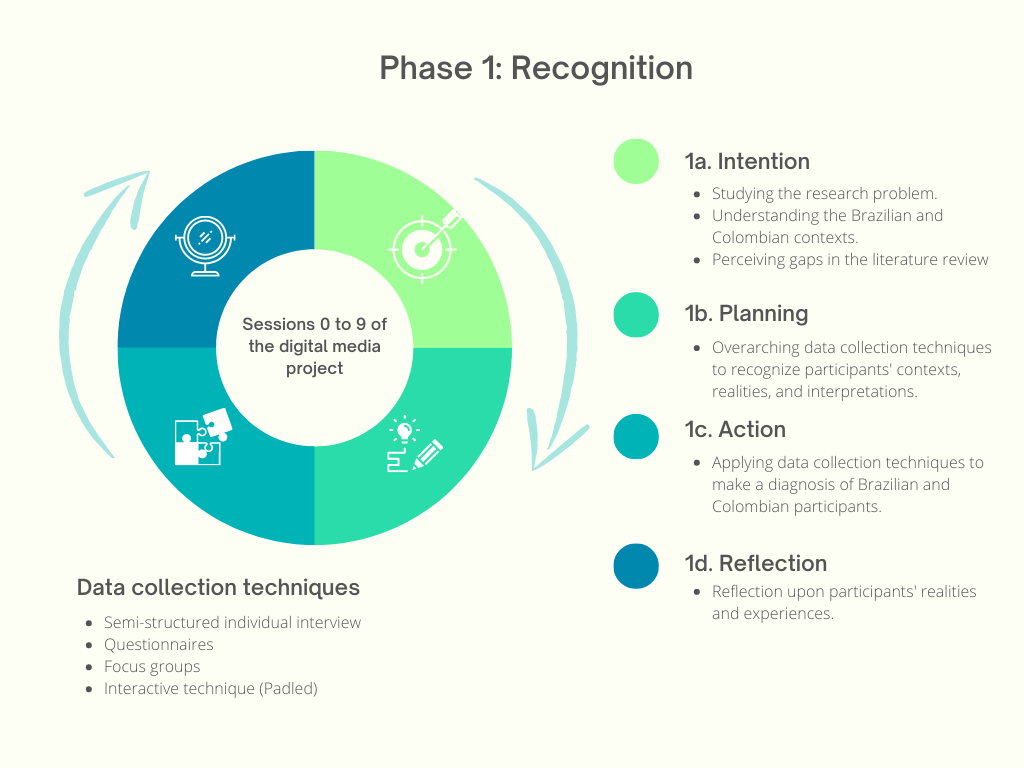
\includegraphics[width=0.8\linewidth]{Fig1.png}
    \caption{Phase 1 of the action research.}
    \label{fig1}
    \source{Own elaboration.}
\end{figure}

Phase 2: We called this session “the action phase”. In this stage, we provided them with a platform to share their personal experiences and engage in meaningful discussions, allowing for the negotiation of their perspectives. It was a collaborative process where participants created their resistance narratives. This exchange of experiences and perceptions enriched their understanding of the complexities inherent in their personal and professional lives (\Cref{fig2}).

\begin{figure}[h!]
    \centering
    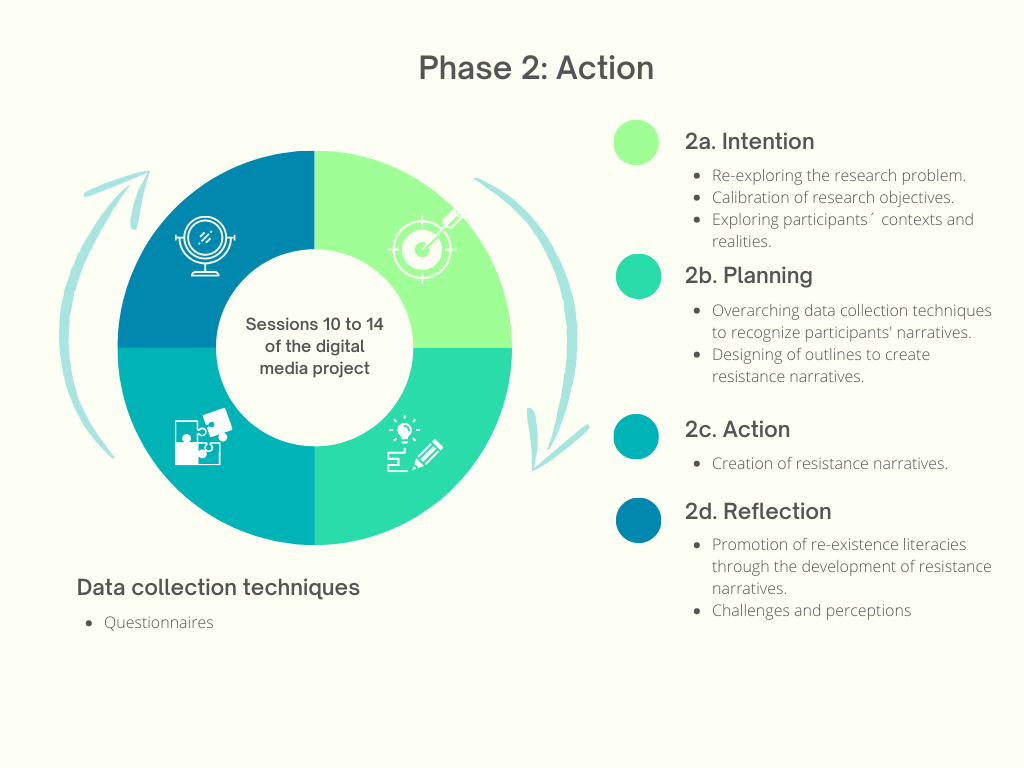
\includegraphics[width=0.8\linewidth]{Fig2.png}
    \caption{Phase 2 of the action research.}
    \label{fig2}
    \source{Own elaboration.}
\end{figure}

Phase 3: We called this step “the evaluation phase”, which marked the culmination of this research project. The primary objective of this phase was to assess and recognise the significance and impact of designing, creating, and implementing digital media projects as critical pedagogy scenarios to promote reexistence literacies among pre-service English teachers. During this phase, careful evaluation and analysis were conducted to gauge the effectiveness of the digital media projects in achieving their intended goals. We examined the extent to which these projects successfully fostered reexistence literacies, empowering participants to challenge dominant narratives, resist oppression, and cultivate critical thinking skills (\Cref{fig3}).

\begin{figure}[h!]
    \centering
    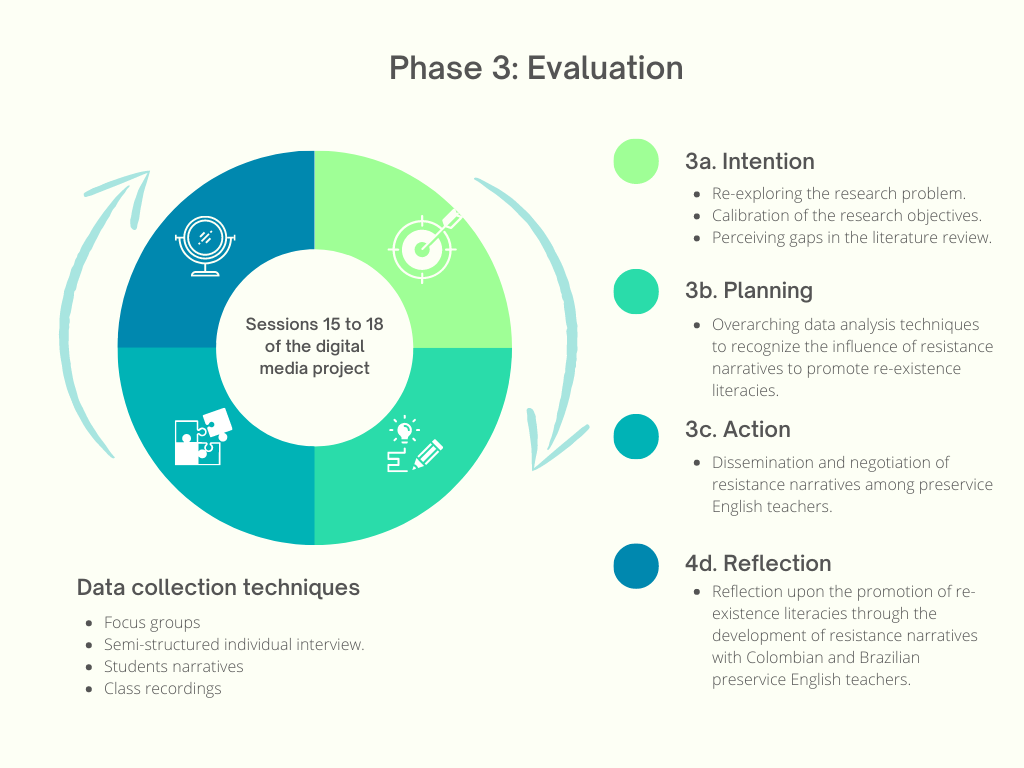
\includegraphics[width=0.8\linewidth]{Fig3.png}
    \caption{Phase 3 of the action research.}
    \label{fig3}
    \source{Own elaboration.}
\end{figure}

For the development of this action, we created an online media project that allowed Brazilian and Colombian students to connect in one place. We used the internet to eliminate the barriers of time and space that could arise between both populations. We understood this media project as a scenario put at the service of preservice English teachers for the creation of their narratives and reflection on their sociocultural practices. Through this exercise, the participants could create resistance narratives that helped them question their contexts and their ways of existing in their worlds.

\subsection{The online media project}\label{sec-organizacao}
We divided the media project into four units: (A) Resistance narratives to promote reexistence literacies, (B) Our role as media users, (C) Taking action, and (D) Thinking twice before making a click. During this exercise, we applied different techniques for data collection, including session recordings, interviews, questionnaires, participants’ resistance narratives, and other techniques that helped guide this process. The media project had 18 sessions, twice a week. Each session lasted approximately two hours. We developed them through the Zoom Platform. Below, we present the generalities of this process (\Cref{tb1}).


{
	\renewcommand{\arraystretch}{1.8}
	\begin{table}[htpb]
		\centering
		\begin{threeparttable}
			\caption{Media Project - General view}
			\label{tb1}
			\begin{tabular}{lp{4cm}p{6cm}}
				\toprule
				Session & Unit & Topic \\
				\midrule
				& NA & General instructions and informed consent \\
				1 & Resistance narratives to promote reexistence literacies & Welcome and diagnostic questionnaire. \\
				2 & & Introduction to resistance narratives. \\
				3 & & Resistance narratives to promote reexistence literacies. \\
				4 & & How do resistance narratives contribute to my reexistence literacies? \\
				5 & & First step: write my resistance narrative. \\
				6 & & Present my resistance narrative idea. \\
				7 & Our role as media users & Our role as media users \\
				8 & & Recommendations to use YouTube as media to liberate. \\
				9 & & Writing the outline of my resistance narrative, part 1. \\
				10 & Taking action & Writing the outline of my resistance narrative, part 2. \\
				11 & & Presenting my resistance narrative outline. \\
				12 & & Video Editors to construct my resistance narrative. \\
				13 & & Video Editors to construct my resistance narrative. \\
				14 & & Media to publish my resistance narrative. \\
				15 & Thinking twice & The privacy of my resistance narrative (Hidden, Private, or Public) \\
				16 & & Socialisation of resistance narratives. \\
				17 & & Publishing my resistance narrative to re-exist. Are you aware of the consequences? \\
				18 & & Evaluating resistance narratives to promote reexistence literacies. \\
				\bottomrule
			\end{tabular}
			\source{Own elaboration}
		\end{threeparttable}
	\end{table}
}



\subsection{Participants}\label{sec-organizacao-latex}
We selected 18 participants to be part of the media project, 11 belonged to the English Language Teaching Program at the Universidade Federal do Piauí, Teresina, Brazil, and 7 belonged to the Foreign Languages Teaching Program at the Universidad Católica Luis Amigó in Medellín, Colombia. This resulted in a percentage of 61.11\% Brazilian students and 38.89\% Colombian participants at the beginning of the research project. 83.33\% of the participants (15) were between 18 and 25 years old, while 16.67\% (3) were older. Among the participants, 11 were men and 7 were women, reflecting the same percentage as before (61.11\% men and 38.89\% women). 36\% of the participants were from a low socioeconomic background, while 60\% reported being from a medium-low socioeconomic background. Only 4\% of the participants reported being from a higher socioeconomic background. This information was calculated using each country's measurement system.

\subsection{The categorisation processes}\label{sec-titulo}
The entire categorisation process arose from the analysis of open and axial decoding. To arrive at this simplification process, we read and reread the data to familiarise ourselves with it and gain a deep understanding of the emerging themes and patterns. We considered the advice of \textcite{miles1994qualitative}, who argue that categories can be merged, divided, or redefined to better reflect emerging patterns in the data (\Cref{tb2}).

\begin{table}[htpb]
	\centering
	
	\begin{threeparttable}
		\caption{The categorisation processes}
		\label{tb2}
	
	\begin{tabularx}{\textwidth}{X X X X}
	
	
			\toprule
				
	\multirow{1}{*}{\textbf{Objective: To comprehend the medias as a critical pedagogy scenario to promote reexis-}}

     \multirow{1}{*}{\textbf{tence literacies in pre-service English teachers}}
		\\
		
	\textbf{Open coding} & \textbf{Axial coding} & \textbf{Category (ies)} & \textbf{Topic} \\
			

		
		Average (dis)advantages & \textbf{Scope/Media project} & Media as a critical pedagogy scenario & Media as a critical pedagogy scenario to explore social issues and challenge dominant power structures \\ 
		Coloniality & Critical pedagogy & Inclusive and resistant environments for English teacher education & Education for Equity: Building Resistant Environments for English Teacher Education \\
		Creation of resistance narratives & Critical media & English teachers and digital media role & Preservice English teachers’ roles in/from media scenarios \\
		Critical English teaching & Critical practice &  &  \\
		Critical literacies & Resistance narratives &  &  \\
		Critical media & Power structures &  &  \\
		Critical pedagogy & Promotion of reexistence literacies &  &  \\
		Critical media & Resistance &  &  \\
		Digital ethics & Social issues &  &  \\
		Digital media consumption & \textbf{Resistance Context and English Education} &  &  \\
		Digital media project & School &  &  \\
		Digital media & Critical English teaching &  &  \\
		Digital practices & English teaching &  &  \\
		English teaching & Negotiations &  &  \\
		Media user role & Realities of the participants &  &  \\
		Negotiations & Resistance &  &  \\
		Power structures & \textbf{Average (dis)advantages} &  &  \\
		Promotion of reexistence literacies & Digital media role &  &  \\
		Realities of the participants & Digital Ethics &  &  \\
		Resistance school & Digital media &  &  \\
		Social issues & Digital media consumption &  &  \\
				& Digital practices &  &  \\ 
				& Critical literacies &  &  \\ 
				&Language Teachers &  &  \\ 
		& Media user role &  &  \\ 
			\bottomrule
		\end{tabularx}
		\end{threeparttable}
		\source{Own elaboration}
	
\end{table}



	


\section{Results}\label{sec-autores}
\subsection{Recognition and perceptions of the context}
When it came to the composition of the participants’ families, we noticed that 72.22\% of them identified themselves as part of traditional nuclear families, while 27.78\% did not. In terms of gender identity, they had diverse identities. The majority, 61.11\%, identified themselves as heterosexuals, while 22.22\% identified themselves as gays and 11.11\% identified themselves as non-binary. Interestingly, a significant portion of the participants (61.11\%) reported being attacked or facing opposition due to their way of thinking or acting. This was the case of Utena, a 24-year-old Brazilian person who considers themself non-binary and who, since childhood, has been a victim of exclusion, rejection, and abuse.

\begin{quote}
    I have faced many dark things due to my gender Identity. As you know I am a nonbinary person. And due to that situation, I had suffered bullying at school. That is why I see myself as an example of those stereotypes and narratives. People cannot see that I am also a good person and they just want to judge. (Utena, Class recording, Session 4, 28:25:00)\footnote{All participant names are fictitious. In fact, they themselves determined how they wanted to be named in this investigation.}
\end{quote}

When we analysed media consumption, 61.11\% of the participants reported engaging in media consumption, while the remaining 38.89\% did not actively consume media. Among the participants, 22.22\% stated that they were aware of their media consumption habits, while the majority, 77.78\%, indicated a lack of awareness. Also, the participants highlighted various purposes for using the media. Learning was a common purpose, with 55.56\% of participants using media for educational purposes. Entertainment also played a significant role, with 66.67\% using media for enjoyment. 5.56\% of the participants mentioned that they used media platforms for socialising, while 33.33\% mentioned that they used media to stay informed about current events. Additionally, 22.22\% of participants specifically mentioned using media for learning English. Interestingly, 11.11\% of the participants identified themselves as “digital content builders”, indicating their involvement in creating digital content for various platforms.

\subsubsection{Perceptions about resistance to reexist}\label{sec-idioma}
Participants expressed various perceptions about the relevance of resistance to reexist. Some highlighted the relevance of pointing out opposition to the abuse of power and oppression as a crucial aspect of reexistence. Others emphasised notions of potency, response, and courage, highlighting the strength required to stand up against challenges. Voice, place, and opportunity were also significant themes, representing the importance of having a platform and the ability to make a difference. Some participants focused on the concept of defining their rules of existence, emphasising autonomy and self-determination in their resistance. Standing up, defence, and force were seen as integral components, demonstrating the resilience and determination required to resist.

Empowerment was another prevalent perception, highlighting the transformative nature of reexistence. Preserving one's voice and resolution were also important factors mentioned, signifying the commitment to staying true to oneself and resolving conflicts. The participants considered these scenarios crucial spaces for supporting political, economic, social-cultural, environmental, and racial issues. They have become a chance to raise our voice, force, and memory, showing the need to remember and learn from past struggles. To show an example, we can see the perception that María, a 22-year-old Brazilian girl, has been a victim of acts of racism and now sees her reexistence as a way to survive and continue fighting against social injustices.

\begin{quote}
    I understand reexistence as the ability to create new ways of telling the story. Stories that are not told or when they are, minorities are placed as wrong or something even worse. It is to create a new way to survive and fight against the system. It's a really exhausting process, but we need to move forward or we will be erased again and again. It's not just about surviving, it's about living freely. (Maria, Padlet, Session 4).
\end{quote}

As Maria did, the other participants emphasised the need to present another part of the story, moving beyond the traditional perspective of victory and acknowledging the complexities of resistance. That is why they recognised the importance of proclaiming the efforts and contributions of individuals in their resistance journey. They also realised the importance of strength, bravery, and overcoming obstacles, showcasing determination and resilience in the face of challenges. It requires the ability to overcome and not repeat past mistakes, emphasising the need to learn from history and avoid the repetition of detrimental patterns. Also, they recognised the importance of determination, persistence, and the ability to break barriers, signifying their unwavering commitment to challenging the status quo. To achieve these competencies, empowerment is a potent symbol of resistance, representing the collective voice and the transformative power of movements.

\subsubsection{Challenges to promote reexistence literacies through the development of resistance narratives}\label{sec-resumo}
During the process of creating resistance narratives through the media project, participants mentioned difficulties in thinking about the resistance narrative itself, organising videos and cutting them, managing external noise, and effectively using video editors. Some participants also faced challenges related to time management, the relevance of the narrative, exporting and downloading the final product, and maintaining video quality. To overcome these challenges, participants provided advice based on their experiences. These included reflecting on personal experiences, watching tutorials before starting, using the intuitive software, adding personal flair to the editing process, organising time effectively, finding a quiet recording space, being patient when editing in a second language, attending additional tutorials, and scheduling activities. Once more, we can see the case of María, who expressed to us all the technical and personal difficulties that she had in developing her narrative and participating in the media project.

\begin{quote}
    When I tried to write my script, I started to think about what happened before in my life, and I was kind of triggered. \textit{Ficaba um pouco gatilhada, um poco travada. Entao pensaba eu nao vou fazer isso hoje, eu nao estou bem para fazer isso hoje. Entao eu parava para pensar e era um proceso demorado. Nao era questao de usar tenologia era porque ficaba gatiliada}\footnote{It was a little triggered, a little blocked. So I thought I'm not going to do this today, I'm not well enough to do this today. So I stopped to think and it was a lengthy process. It wasn't a question of using technology, it was because I was triggered (Our translation).}. (Maria, Semi-structured Interview 2, Session 18)
\end{quote}

We identified that 70\% of participants expressed concerns about sharing their personal experiences and the potential for facing judgment or negative comments. Despite this, around 80\% of participants recognised that creating resistance narratives allowed them to learn from their own cultures and the cultures of others. This process of self-reflection and understanding led to personal growth and an expanded sense of reality. Furthermore, around 75\% of participants acknowledged that creating resistance narratives fostered cultural and personal exchanges. However, according to Alexis de Palma, a young English teacher training at the Federal University of Piauí, who identified themself as gay, when we are going to spread a narrative of resistance, it is necessary to consider the pros and cons of this exercise.

\begin{quote}
    Sometimes you are not prepared emotionally, because you can receive a lot of bad comments about your resistance narrative. You need to know some people are gonna tell you some bad words, but at the same time, you can find a lot of people that are going to support you. (Alexis de Palma, Semi-structured Interview 2, Session 18)
\end{quote}

By sharing their stories, participants could connect with others, learn about different perspectives, and promote their culture. This interaction with diverse narratives not only enriched their understanding but also allowed them to negotiate and share experiences with people from different backgrounds. However, it is important to note that the creation of resistance narratives was not without its disadvantages. Approximately 60\% of participants mentioned the potential to offend others' sensibilities, encounter prejudices, or face discrimination. The exposure to cyber hate, censorship, and the risk of misrepresentation were also concerns expressed by participants. Due to the development of this media project, the participants developed a greater awareness of the diffusion and reception of information. This is the case of Beatriz, another 22-year-old Brazilian girl who showed us how this exercise managed to transform her.

\begin{quote}
    Agora eu tenho mais atencao nas coisas que eu falo, as coisas que eu posto para nao perjudicar ou ofender ningem. Agora eu sou mais ciente do conteudo que eu estou consumiendo e o que eu estou produzindo. O projeito mediatico me ajudou a refletir sobre isso\footnote{Now I pay more attention to the things I say, the things I post so as not to harm or offend anyone. Now I'm more aware of the content I'm consuming and what I'm producing. The media project helped me to reflect on this (Our translation).}. (Beatriz, Semi-structured Interview 2, Session 18)
\end{quote}

The benefits of creating resistance narratives were substantial. Participants reported increased awareness of their struggles and the struggles of others, as well as a deeper understanding of their own identity and the complexities of human experiences. Additionally, around 80\% of participants recognised the power of resistance narratives as a tool for empowerment, motivation, and the pursuit of a more just and fairer world. The process of creating resistance narratives presented both challenges and opportunities for participants. While the potential for negative experiences and backlash existed, the overall impact was positive, leading to personal growth, cultural exchange, and the dissemination of important stories. The power of resistance narratives to inspire, educate, and connect individuals cannot be overlooked, as they contribute to a more inclusive and empathetic society.

Approximately 70\% of the participants mentioned that they acquired proficiency in video editing, merging audio and video, and using new apps for editing and expressing their opinions, which were the most prominent categories of new knowledge and literacies related to digital skills and technological literacy. These technical skills enabled them to harness the power of digital media for self-expression and storytelling. Also, cultural and linguistic knowledge was another prevalent area of growth; this knowledge expansion fostered a sense of pride in one's identity and a recognition of the diversity of perspectives and cultures that exist in the world.

The development of reexistence literacies was a common theme among the participants, with nearly 80\% expressing personal growth, empowerment, and a deeper understanding of their own stories and identities. They recognised the importance of narratives and storytelling as powerful tools for self-discovery, reflection, and connecting with others who have similar experiences. This was the case of Oróstegui, another 31-year-old young man, who showed us his Colombian reality and how the media project has helped him to understand these realities.

\begin{quote}
    Media could become scenarios to help people who are silenced or pressed. For example, in the protest here in Colombia, the government tries to hide the truth. The problem here in Colombia is two channels manipulate the information. With our social media, we can show another version of the story. (Oróstegui, Semi-structured Interview 2, Session 18.)
\end{quote}

Also, the desire to create resistance narratives and challenge societal norms was strong among the participants, with an overwhelming majority (over 90\%) expressing a commitment to using their newfound knowledge and literacies to raise their voices and negotiate their realities without oppression. They emphasised the importance of addressing ongoing social issues and striving for a more equitable and inclusive society.

Thus, the participants' journey of acquiring new knowledge and literacies, along with the development of reexistence literacies and the creation of resistance narratives, reflects a collective transformation. The percentages indicate a high level of engagement and successful outcomes, suggesting that the learning experiences provided meaningful and impactful opportunities for personal and societal growth. From this perspective, the analysis demonstrates the power of education and learning to foster personal empowerment, cultural understanding, and a commitment to social change. It highlights the participants' remarkable progress in acquiring new skills, deepening their self-awareness, and harnessing their voices to challenge prevailing narratives and shape a more inclusive and just world.

\section{Discussions and conclusions}\label{sec-secoes}
\subsection{Media as a critical pedagogy scenario to explore social issues, and challenge dominant power structures}
Through this research, we could identify that, in English language teaching, integrating innovative pedagogical approaches is crucial for fostering critical consciousness and empowering pre-service teachers to become agents of social change. One such approach that holds tremendous potential is the utilisation of digital media projects. By embracing this approach, educators can impart language skills and cultivate reexistence literacies among pre-service English teachers.

Digital media projects provide a dynamic platform for participants to engage in critical dialogue, explore complex issues, and challenge dominant power structures. In an increasingly interconnected and technologically driven world, digital literacy has become an essential skill for individuals to navigate and critically analyse the vast array of media content they encounter in different languages \cite{garcia2023}. By leveraging digital media in pedagogical practices, educators can equip pre-service English teachers with the necessary skills to navigate the digital landscape critically, empowering them to decipher the underlying messages and power dynamics within media texts.

We also noticed that the use of digital media projects not only fosters critical digital literacy but also encourages participants to reflect on their own beliefs, values, and biases. Through active engagement with various digital media platforms, we expose participants to diverse perspectives and worldviews, which prompts them to question their assumptions and challenge preconceived notions. This process of critical reflection cultivates a deeper understanding of social issues, dismantles stereotypes, and encourages empathy and cultural sensitivity. During this construction, it was possible to demonstrate how the development of this media project contributed to the participants being more aware of their physical and digital interactions. It was significant to see how participants like Max managed to identify the ideologies of the texts that are disseminated on the Internet.

\begin{quote}
    Now, I'm watching some videos and I think about who is involved, what is the video promoting, who is the video against, or what is this video for. I can’t think about it before. I never reflect on this stuff that I see on the internet, but now, I can see it every time. (Max, Semi-structured Interview 2, Session 18)
\end{quote}

Moreover, digital media projects provide a medium for pre-service English teachers to express their narratives and reexistence. By creating and sharing their stories through digital platforms, participants can amplify marginalised voices, challenge oppressive systems, and reclaim their agency. These projects offer a space where alternative narratives can flourish, empowering individuals to shape and reconstruct their identities while celebrating their unique experiences and perspectives.

The incorporation of digital media projects into English language teaching transcends traditional instructional boundaries and aligns with the principles of critical pedagogy. By actively engaging with digital media, pre-service teachers develop a critical lens through which they can analyse and question dominant power structures, biases, and inequities. They become equipped with the tools necessary to challenge societal norms, advocate for social justice, and promote equitable opportunities for all learners.

In this way, the integration of digital media projects as a critical pedagogy scenario in English language teaching opens up new avenues for fostering reexistence literacies among pre-service teachers. By leveraging the power of digital media, educators can cultivate critical consciousness, empower learners to challenge dominant power structures and promote social justice and equity. As we continue to explore and expand such practices, we can create transformative educational experiences that not only enhance language proficiency but also empower pre-service English teachers to become change agents in their classrooms and communities.

\subsection{Critical education for equity: building resistant environments for English teacher education}\label{sec-format-simple}
With this study, we could identify that when education is used to promote equity, resistance, and reexistence, it may generate opportunities for inclusion and transformation to foster cultural identity, community empowerment, and sociopolitical awareness. However, to achieve these outcomes, it is important to consider the narratives of each individual and society as crucial instruments for embracing cultural identity and social diversity and valuing the richness of different cultures. By using media for these purposes, social stigmas and stereotypes are challenged, turning these tools into an opportunity for individuals to reinvent themselves and enjoy a more just and equitable world.

The construction and dissemination of media projects to create resistance narratives helps individuals overcome adversities and gain the resilience necessary to thrive in a more understanding world. By navigating social pressures and maintaining authenticity, individuals can resist oppressive structures and contribute to the creation of a more inclusive and just society. Their stories inspire others to embrace their identity and confront their challenges. This was evident in this project, as it became clear that when an individual seeks support and learns from others with similar realities, it fosters humanistic social relationships based on empathy, peace, and understanding. This sense of unity promotes a supportive environment where the diversity of voices is respected and collective resistance and reexistence can flourish.

For this reason, while this study is not a manual for solving the social problems our students face, it provides an opportunity for reflection and proposes a practice that is useful to be critically examined to address these obstacles and provide supportive environments that empower individuals to confront and resist systemic barriers. This can be evidenced through Harriet's speech, a Colombian non-binary, who invites us to continue working on the development of this type of project to continue fighting for equity and social justice. According to Harriet, we need to find critical spaces to reexist, and this media project became a place to reflect on their reexistence and find other people to build, share, and negotiate their experiences and realities. (Harriet, Semi-structured Interview 2, Session 18).

Therefore, this endeavour is worthy of criticism as we continue to search as an educational community for elements that help equip pre-service English teachers with the tools to analyse and question information critically, resist manipulation, and instil the importance of contributing to a more informed and just society. By overcoming these obstacles, we can speak of a resurgence of resistance that enables individuals to challenge oppressive systems and advocate for social change. Thus, we can empower future educators to become consultants equipped with the tools to challenge oppressive systems, promote equity, and cultivate transformative physical and digital educational spaces.

\subsection{Preservice English teacher’s role in/from media scenarios}\label{sec-links}
We can conclude that the role of teachers in using media scenarios is essential for guiding and supporting students in the critical use of media. As educators, our first task is to provide students with the necessary tools to analyse and question media messages and content reflectively. This involves constantly teaching ourselves how to use digital tools and platforms efficiently and safely and evaluating the reliability and truthfulness of online information. We must learn to discern between different sources of information and recognise the biases and manipulations that may be present in the media.

By developing these foundational skills (literacies), we foster critical awareness regarding the messages and power structures present in the media. From there, we must be able to identify how certain social groups are represented in the media, how stereotypes and prejudices are perpetuated, and how we can challenge and resist these representations. All of this is done to learn to recognise dominant discourses and question them from a critical and reflective perspective. Thus, “if we create social media, we also have to evaluate our role and our responsibilities as being on the internet. It could be so powerful but also so dangerous" (Max, class recording, Session 7, 30:52:00).

Via developing critical and reflective perspectives, we can encourage active participation from our students in creating and disseminating their narratives through digital media. Therefore, as teachers, we can encourage our students to use digital tools to share their stories, perspectives, and unique experiences. This might not only help them develop communication and expression skills but also empower them to amplify marginalised voices and challenge oppressive systems. Students may use the media as a platform to promote diversity, inclusion, and social justice. These uses, as seen in this research, can help an educational community create a safe and supportive environment where students feel comfortable sharing their ideas and opinions about the media. This creates an open and respectful dialogue where their realities and contexts are valued and heard.


\printbibliography\label{sec-bib}
% if the text is not in Portuguese, it might be necessary to use the code below instead to print the correct ABNT abbreviations [s.n.], [s.l.]
%\begin{portuguese}
%\printbibliography[title={Bibliography}]
%\end{portuguese}


%full list: conceptualization,datacuration,formalanalysis,funding,investigation,methodology,projadm,resources,software,supervision,validation,visualization,writing,review
\begin{contributors}[sec-contributors]
\authorcontribution{Edison Ferney Castrillón Ángel}[conceptualization,methodology,datacuration,investigation,visualization,writing,review]
\authorcontribution{Beatriz Gama Rodrigues}[datacuration,supervision,visualization,validation,investigation,formalanalysis,review]
\end{contributors}


\end{document}